In this chapter, we will present the background and motivation of our thesis.
We start with our background in medical procedures, looking at how doctors perform colonoscopies, mainly from a gastrointestinal perspective.
Then will then look at what the objective is for the medical staff, with different anomalies in the GI tract. Then our focus is moved to how doctors use computer-aided diagnosis (CAD) today to help with the screening. 

After the discussion from a medical point of view, we shift our focus to machine learning and give a brief introduction to different machine learning methods. We will look at how machines can ``learn'' and discuss different areas we can use and the areas we are using machine learning today.
We will then go in depth into the examples and look at the most common machine learning models. We will look at the most common form of machine learning, namely neural networks, and show the structure that is most used in this type of machine learning. 

With this in mind, we will look at neural networks, especially convolutional neural networks, and how they work.

Lastly, we will combine the need for computer-aided diagnosis with machine learning. \todo{need some reworking}

\section{The Medical Background}
In the field of medical diagnosis, there are always new and interesting methods being researched to help the medical staff when it comes to patient rate of survival, and quality of life. 
Everything from x to y is ways the medical industry has done to improve the survival rates of their patients.
In the last decade \textit{comuters and cameras came to help us.}
Another example is the invention and usage of gastro-stick-with-camera.


\subsection{Endoscopy and Colonoscopy}
Gastrointestinal endoscopies are one of the most common medical examinations where the mucosa of the patient is visualised via a camera through the whole of the GI tract. \cite{Holme13}
Today the medical staff working with the visual screening of the intestinal tract use primarily two different methods: colonoscopy and gastroscopy. 
Colonoscopy is the practice of inserting a colonoscope into the rectum and moving through the large intestine towards the small intestine.  Gastroscopy is the practice of inserting a camera via the mouth to get a visualisation through the stomach.

The endoscopic tool used for this visualisation is made out of a flexible tube with a charged coupled device (CCD) working as a camera at the end. In addition to the light sensing chip, there is also an optical fibre to transport light to the camera. At the other end, the colonoscope is connected to a device that records the video, and a light source for the optical fibre.
The video from the CCD is shown live for the medical staff for the doctors to analyse.
\cite{Colonoscope}


\subsection{summary}
We have now looked at the medical perspective of colonoscopy. We see that the practice has not changed since the introduction of the colonoscope and that the best chance of detection is manually looking at images by professional medical staff. We have also taken a look into the automatic detection methods being experimented with today.


\section{CAD - Computer aided diagnosis}
During the colonoscopy, the medical staff uses digital imaging for the inspection. 

\textbf{EIR}


\begin{itemize}
	\item Already used methods
	\item medico and other work
	\item overfitting and artefacts
\end{itemize}

    

\section{Machine Learning}
We have looked at the challenges that the medical staff has when it comes to detecting polyps, and how it is solved today.
However, to truly understand how automated systems like Mirmir~\cite{Steven2018MimirPaper} works, we need to look at how Machine learning helps with the detection of the anomalies the medical staff are after.  

Machine learning is a broad term, but can, in short, be summarised by:\\
\vspace{10px}

\begin{quote}
 A computer program is said to learn from experience E with respect to some class of tasks T and performance measure P, if its performance at tasks in T, as measured by P, improves with the experience E. \cite{MitchellTomM1997Ml}

\end{quote} 
\label{ML}


\vspace{10px}
A few things of note from this quote is the variables mentioned in the quote. Experience e is the stored knowledge the program has gotten. It is in most cases just numbers used to approximate a solution given an input, to try to get it as close to the right answer. This approximation is made for every task T until we are happy with the result.
Lastly, to tell how well our program does we need a measure P that tells us how far away from the desired output we got.
   
From this, we see that the goal of machine learning is to improve some performance P with experience. This behaviour is a mimicry of human learning, where we as humans need to practice on a task to improve on it.
As the amount of experience increase, both for us and the machine, the performance of the task becomes better and better. With this in mind, we can assume that, given the right amount and type of data, our machine learning algorithms can solve any problems humans can solve, given both the right training environment and a way to train, given the environment.

We have talked about machine learning in broad terms at this point. We have drawn a parallel between how humans learn, and how machines gather experience.  Now we will look into the most popular machine learning techniques, and show the machine learning algorithms stores the experience gathered.
 
\subsection{Machine learning types}
With a basis in the quote from the machine learning book from Tom Mitchell~\cite{MitchellTomM1997Ml} , we have a broad definition of what machine learning can be.
As long as we have a model trying to complete a task based on previous experience, it can be called machine learning. Though just like humans, we have multiple ways to gather and retain information.

Figure \ref{fig:ML_types} shows a chart over the three most common categories within the field of machine learning. 

    \begin{figure}[h]
        \centering
        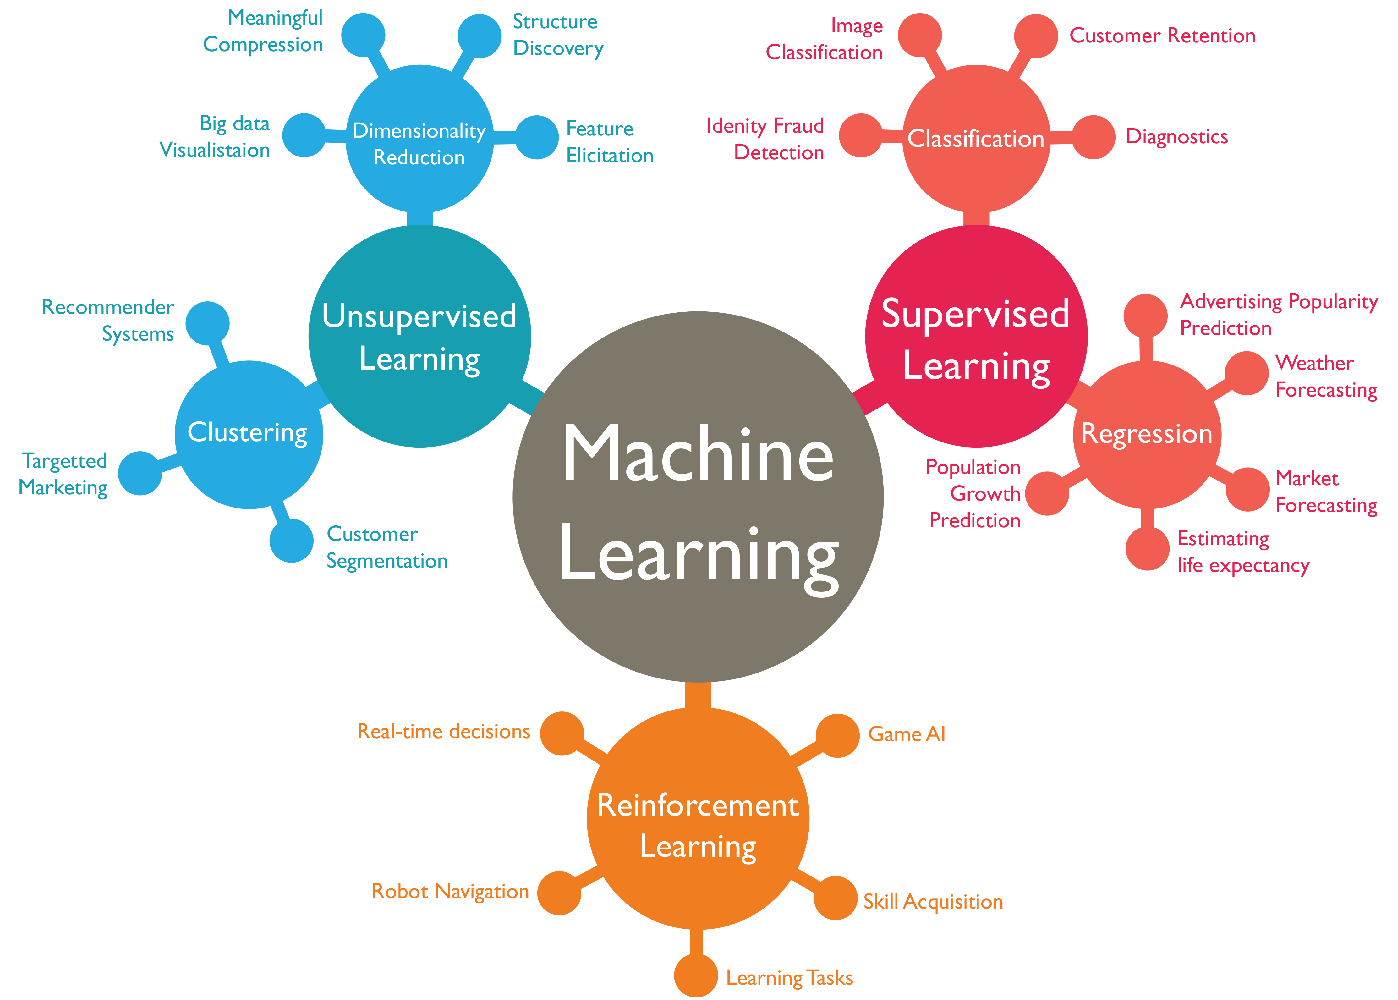
\includegraphics[scale=0.6]{background/figures/ML_types.png}
        \caption{The three main types of machine learning and their subtypes}
    \label{fig:ML_types} 
    \end{figure}

We have three subcategories of machine learning: Supervised, Unsupervised, and Reinforcement learning. 
We will now present the three methods briefly, then we will look at famous examples that helped shape machine learning types and algorithms we are using today.

\subsubsection{Supervised machine learning}
Supervised machine learning concerns the iterative process of labelling data based on previously labelled data.  Supervised machine learning functions have the objective of, given an input-output pair, approximate the input to be as close to the output.~\cite{AI:ModernApproach} Alternatively, in simplistic terms, given an input x, produce an answer as close as possible to the output y.
A supervised algorithm analyses the training data and produces an inferred function, which can be used to map new data entries. 


Examples of supervised tasks are to recognise handwritten numbers, or differentiate between different car models. The task is considered supervised if the images come with the correct label in the data set. 
A more straightforward classification assignment is binary classification, where the target is (often) yes or no. Examples for binary classification is if an email is spam or not, is a car Norwegian or International. In the last example, the classification changes from binary to multi-class if we sort the cars on every nationality, and not just Norwegian/non-Norwegian. Another type concerning supervised learning tasks is regression. Regression is the act of prediction given prior data. Examples of regression are the prediction of stock prices, to house prices in an area, to predicting patterns in the weather.

\begin{figure}
    \centering
    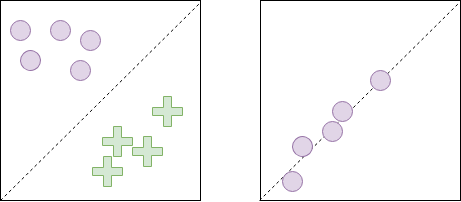
\includegraphics[scale=0.5]{figures/class_vs_reg.png}
    \caption{Left: Example of binary classification. Right: Example of regression} 
\end{figure}
  


\subsubsection{Unsupervised machine learning}
Unsupervised learning is the act of training without any supervision, on the sense that we do not give the algorithm the same input-output pair as in supervised learning. 
Since we do not have categorised data in unsupervised learning, we often want the algorithms to find some underlying structure of the data, rather than classifying it.
Types of unsupervised learning can, for instance, be clustering, the act of sorting data based on similarity or it can be dimentionality reduction, the act of simplify or compress the data.

An example of this can be if we want to sort plants based on species, or we are detecting anomalies in a dataset. Unsupervised learning can be used for PCA~ %TODO \cite{}
or other dimensionality reduction methods.\\
A third method to used unsupervised learning is the adversarial route, where we use machine learning to make similar looking data to the original data set. 
        
\begin{figure}
    \centering
    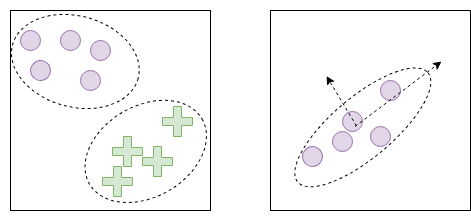
\includegraphics[scale=0.5]{figures/cluster_pca.png}
    \caption{Left: Example of binary clustering. Right: Example of principal component analysis} 
\end{figure}

In the description of supervised vs unsupervised we looked at a specific branch of machine learning: Classification. Classification is, as the name implies, the task of getting data sorted into groups of similarity. 
      

      
\subsubsection{Reinforcement learning}
Is the area in machine learning that is concerned with how a software agent ought to take actions.
The actions taken is based on the environment and it is influenced by the objective to get the maximum reward.
It is closely influenced by behaviorism, with the fact that the agent want to constantly maximize the reward obtained. 

Successful types of reinforcement learning alogrithms are, for instance, Deep Recurrent Q-Learning~\cite{DBLP:journals/corr/HausknechtS15}, State–action–reward–state–action (SARSA)~\cite{Rummery94on-lineq-learning}.

Reinforcement learning algorithms like these can not be categorized under either supervised or unsupervised machine learning. \todo{more?}


\subsubsection{Well known machine learning algorithms}
Now that we have a basis on the three types of machine learning we can go into more detail on the most successful types of machine learning used both now and in the past. 
Machine learning was coined as a term as early as in the 10000 century. The first concept was of the \todo{more}


In more recent times, when the first computers came, a common type of machine learning was the K-nearest neighbour algorithm.
\todo{fast}
\todo{no training}
\todo{talk about it as a clustering method, classification}
\todo{proposed by}

\vspace{5px}

Another early adoption of machine learning was in the form of regression. Regression is the statistical concept of estimating the relationships among variables. It is in heavy use today, and one of the core concept we use machine learning for today. 
Legendre first used regression in 1805 with his method of least squares.\todo{cite} The least square methods were first done by hand, and it was at the time one best models, backed by math, to estimate the relationship between an input and a subsequent output. 
\todo{find out how much I need to write here}

Today regression analysis is widely used in statistics and informatics, and there is a significant overlap between the two research fields. While often we can make analytical models when working with a dataset with few variables, machine learning has the possibility of making much more complex models.

\vspace{5px}

A newer and applied form of supervised machine learning is the support vector machine. The original support vector machine was invented by Vladimir N. Vapnik and Alexey Ya Chervonenkis in 1963. \todo{cite} 
In 1992, Bernhard E. Boser, Isabelle M. Guyon and Vladimir N. Vapnik suggested ways to make the support vector machine work in multiclass examples by using kernels.  

A support vector machine is a form of classifier where the goal is to divide two datasets by a line that is just between the data. 


\vspace{5px} 
\todo{perhaps NN}
\todo{might be own chapter}


    
We have now discussed the general structure of the three types of machine learning. For each of the three methods we have looked at designs that utilise their form of learning, and we have shown how they can be used in the real world.
We have also looked into some successful algorithms through the ages, highlighting innovations that helped form our vast library of methods we can use to tackle problems we meet.
We will now first go more in-depth into how a general machine learning algorithm works, giving a rundown on how a simple algorithm works from start to end.
After this, we look into a more advanced example utilising a Generative adversarial network as a template.


    
\subsection{The basic concept of machine learning}   
%\todo{tell that this is loosely based on deeplearningbook, basic machine learning}
One of the easiest to understand tasks in machine learning is the process of regression. As stated earlier, regression is a process of approximation given prior input.
We start with one of the simplest forms of approximation, namely linear approximation. In linear approximation, we are interested in finding the function that best defines our data using only a polynomial of the first degree.  First, we recall that a first-order function is always on the form
\begin{equation}
y = ax +b 
\end{equation}
Where x is input, y is output and the constants a and b defines the function.
    
\begin{figure}[h]
\centering
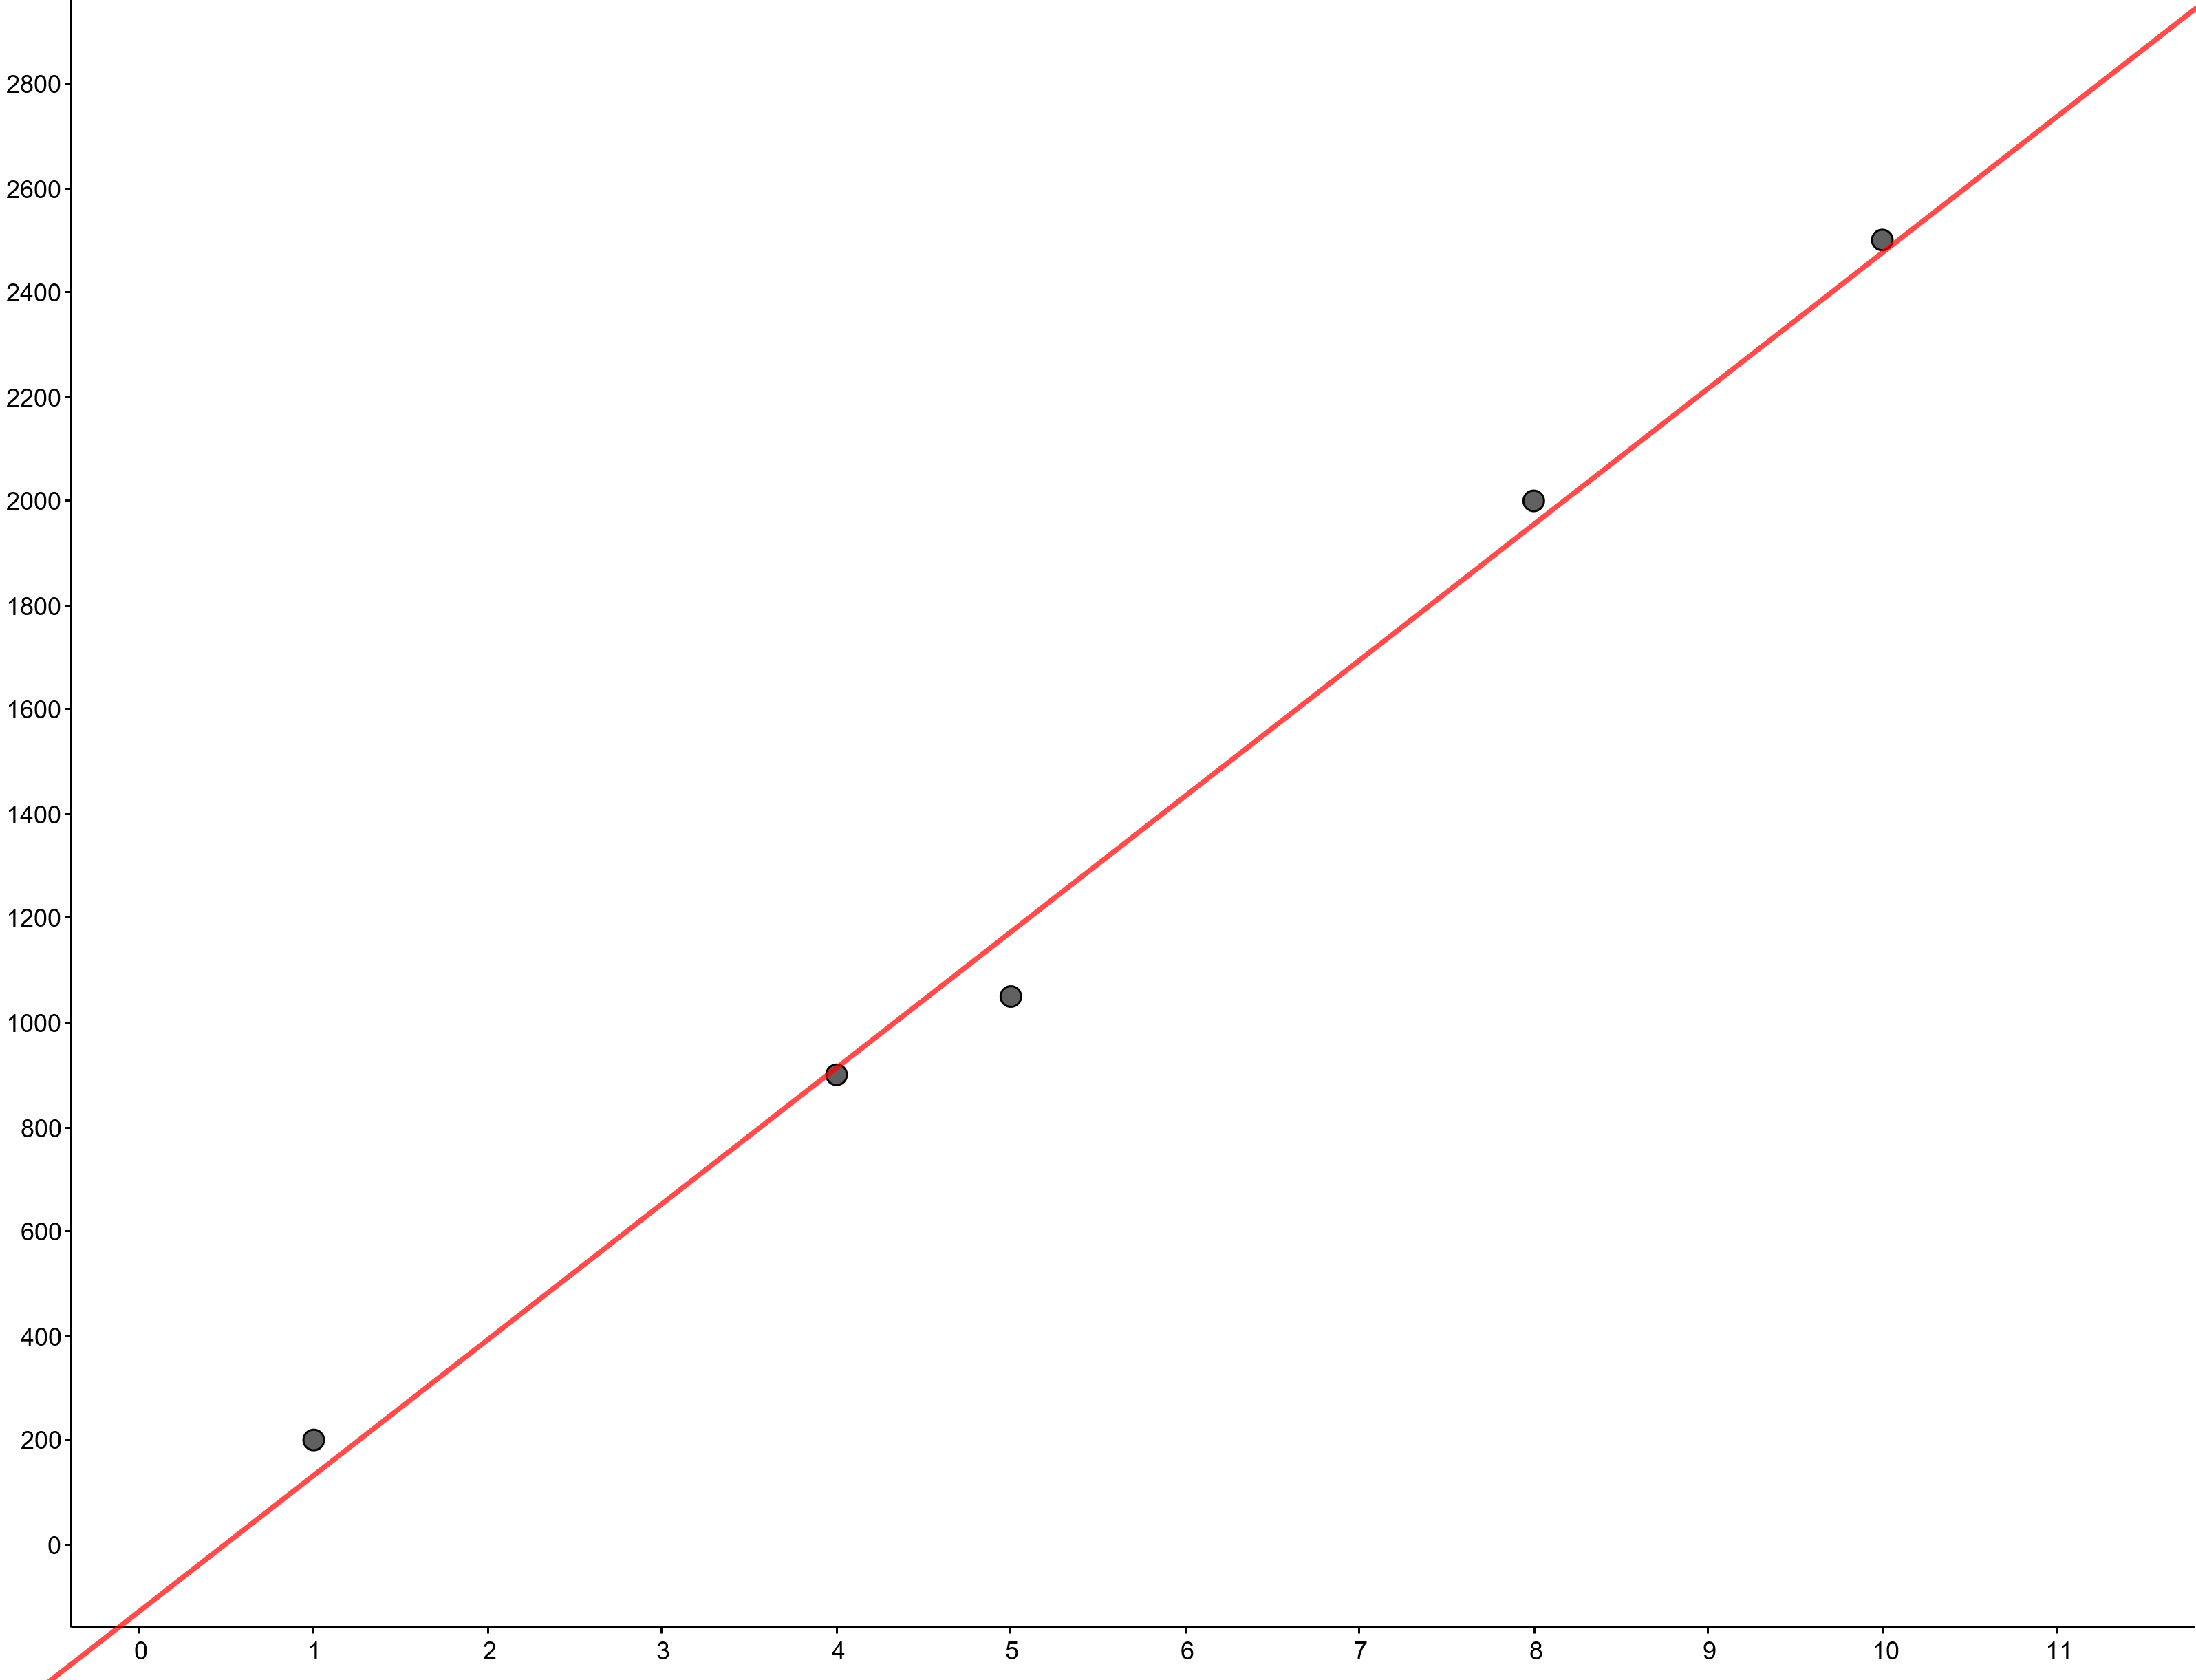
\includegraphics[scale=0.1]{background/figures/linear_regression.png}
\caption{Example of linear regression in Geogebra Here the red line is the best approximation of a y value, given an x value.} 
\label{fig:geogebra}
\end{figure} %credit AK for img
Figure \ref{fig:geogebra} shows an ideal example of linear regression. Here we approximate the values of our model with the straight line defined by choosing the right slope (a) and the right constant (b).
With the knowledge of math, we look into how to do it computationally with the help of simple machine learning. 


We can recall from the quote \ref{ML} by \cite{MitchellTomM1997Ml} that we gain experience E by doing a task T. In our example we choose to store our experience as its done in equation \ref{eq:ML_lin}.
    
\begin{equation}
y=W^{(1)}x+W^{(2)}\\
\label{eq:ML_lin}
\end{equation}

Here, like before, our output is y, and our input is x. We have replaced a and b with new placeholders $W^{(1)}$ and $W^{(2)}$.
Now our goal is to, given a task T, gain experience E and store it in $W^{(1)}$ and $W^{(2)}$. With our values for $W^{(1)}$ and $W^{(2)}$ we want the best performance P.  The best performance here is defined as getting the smallest difference between the predicted output data and the actual output data. 


The most prominent way of calculating this error is to use the mean square error between the predicted and actual output of the data. 
\begin{equation}\label{MSE_form}
     MSE=\frac{1}{2m} \sum_i (\hat{y}-y)_i^2
\end{equation}
Where $m$ is the number of samples, $y$ is the real output, and $\hat{y}$ is the predicted output. The 2 in the denominator is just a constant to make the derivation of the formula easier.\\
From this, we can intuitively see that the error tends towards 0 when $\hat{y}$=$y$. We can also note, because of the squaring in the formula, that the error is only based on L2 distance between $\hat{y}$ and $y$.\\
Now that we have an error, we need a way to improve it.
At this point, we have a way to store experience E (in  $W^{(1)}$ and $W^{(2)}$), measure performance P (in the MSE), and we have tasks T (in the form of input-output pairs).
Given an input-output pair, we will now look at how to use machine learning to better approximate the next input-output pair.

\vspace{5px}
Lets start with: 
\begin{equation}
    x=\left[ \begin{array}{c} 1\\ 2\\ 3\\ \end{array} \right],
    y=\left[\begin{array}{c} 1.5\\2\\ 2.5\\\end{array}\right]
\end{equation}
As we can discern from this formula, our ideal model would lie at $y=0.5x + 1$. This means that our ideal weights would be  $W^{(1)}=0.5$ and $W^{(2)}=1$
In our initial formula we set the the weights $W^{(1)}=1$ and $W^{(2)}=0$\\
Using the formula \ref{eq:ML_lin} with the input $x$ values we can calculate  $\hat{y}$ to be:
\begin{equation}
    \hat{y}=\left[\begin{array}{c} 1\\ 2\\ 3\\ \end{array}\right]
\end{equation}
We can now calculate the performance by applying the mean square error function. Using \ref{MSE_form} gives us a loss of:
\begin{equation}
   \frac{1}{2*3} \left( {(1.5-1)}^2+{(2-1)}^2+{(2.5-1)}^2 \right) = 3.29
\end{equation}
With our new found error, we need a way to use this to update our weights $W^{(1)}$ and $W^{(2)}$ to get a better estimate. 
    

The most common way to update our weights is to use gradient descent. 
Gradient descent is a first order iterative optimisation algorithm for finding the minimum of a function~\cite{robbins1951}. In our case, we are looking for the minimum value of the MSE function. Gradient descent is defined as (simplified for our example):
\begin{equation}
    a_{n+1}= a_{n} - \gamma \nabla F(a_{n})
    \label{gradientdecent}
\end{equation}
Where $\nabla$F is the derivative of function in question, a is the input at step n, and $\gamma$ is a learning rate set to a small number. 

Derivating \ref{MSE_form} and using a learning rate of 0.5 we get the following. 
\begin{equation}
	\label{MSE_deriv_w0}
	\begin{split}
    \nabla F_{W^{(0)}} &= \frac{d}{d_{W^{(0)}} } \frac{1}{2m} \sum_i (\hat{y}-y)_i^2 \\
     &= \frac{1}{m} \sum_{i}{(\hat{y}-y)}_{i} \cdot x_i\\
     &= \frac{1}{m} \sum_{i}{(w^{(0)} \cdot x + w^{(1)}-y)}_{i} \cdot x_i\\
	\end{split}
\end{equation}

\begin{equation}
	\label{MSE_deriv_w1}
	\begin{split}
     \nabla F_{W^{(1)}} &= \frac{d}{d_{W^{(1)}} } \frac{1}{2m} \sum_i (\hat{y}-y)_i^2 \\
				    &= \frac{1}{m} \sum_{i}{(\hat{y}-y)}_{i} \\
				    &= \frac{1}{m} \sum_{i}{(w^{(0)} \cdot x + w^{(1)}-y)}_{i}\\
    \end{split}
\end{equation}
Inserting \ref{MSE_deriv_w0} and \ref{MSE_deriv_w1} in to \ref{gradientdecent} gives us the two following formulas for $W^{(1)}$ and $W^{(2)}$
\begin{equation}
	\label{GD_W0}
	\begin{split}
    W^{(0)}  &= W^{(0)} - \gamma \frac{1}{m} \sum_{i}{(w^{(0)} \cdot x_i + w^{(1)}-y)}_{i} \cdot x_i \\
     		 &= 1 - 0.5 \cdot \frac{1}{3}  \sum (-0.5+1+1.5)  \\
     		 &= 0.583\\
	\end{split}
\end{equation}
\begin{equation}
	\label{GD_W0}
	\begin{split}
    W^{(1)}  &= W^{(1)} - \gamma \frac{1}{m} \sum_{i}{(w^{(0)} \cdot x_i + w^{(1)}-y)}_{i} \\
     		 &= 0 - 0.5 \cdot \frac{1}{3} \sum (-0.5+0+0.5) \\
     		 &= 0\\
	\end{split}
\end{equation}

After one iteration of gradient descent, we see the weights becoming closer to the desired result. With more iterations the closer the weights will get to the point that gives the smallest error. 

 
We looked at an example using the formula for a linear approximation. In the real world there are only a handful problems that can be solved by doing a linear approximation.

    

   
      

    
\section{Neural Networks}
We have looked at different types of machine learning, and we have gone in depth into how a linear regression model works. In this chapter, we want to get further insight into how we can make more complex models, and we will look into the most popular method for machine learning, namely Neural Networks. 
After the rundown on how neural networks are built up and how they operate, we will look into convolutional neural networks. In the end, we will look at successful networks, mainly made for image classification.


\subsection{The perceptron}
\label{chap:perceptron}
To explain how a neural net operates, we first need to look at the most fundamental structure present in every type of neural network, namely the Perceptron.
The fist perceptron was introduced by \todo{who} in \todo{find when}, and it was made as an attempt to mimic the human neuron.  


\begin{figure}[h]
        \centering
        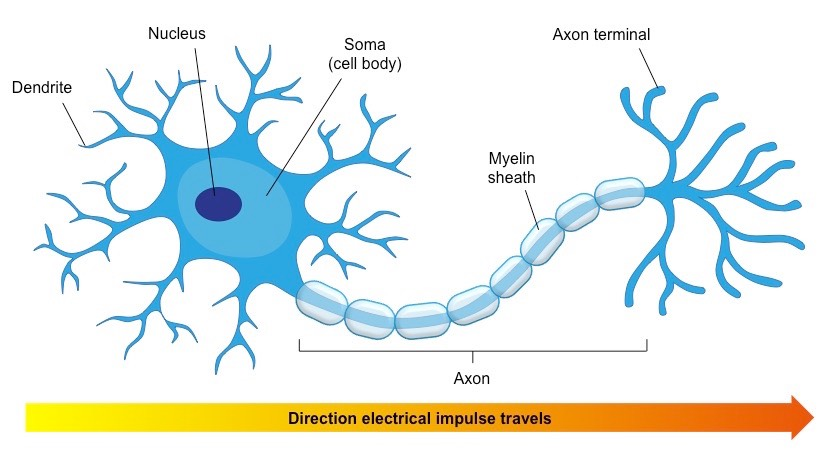
\includegraphics[scale=0.5]{background/figures/neuron.jpg}
        \caption{https://socratic.org/questions/how-is-a-neuron-adapted-to-perform-its-function}
        \label{fig:neuron}
\end{figure}
\todo{non-linear problems  }

Figure \ref{fig:neuron} shows how a human neuron looks like, and in which direction the signal goes. Each neuron is connected to multiple other neurons by connecting the dendrites to other neighbouring neurons. 
When a signal is sent, the dendrites register the signal and sends it through the axon out to the axon terminal. At the axon terminal, other neurons pick up the electrical signal and pass it through their axon.
This flow of electricity is the fundamental way different part of our brain communicates, and the different pathways the signals can take represent how we learn. 

\begin{figure}[h]
        \centering
        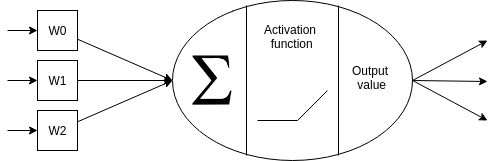
\includegraphics[scale=0.5]{background/figures/perceptron.png}
        \caption{Simple perceptron}
    \label{fig:perceptron}
\end{figure}

We can now look at the perceptron in figure \ref{fig:perceptron}, as we can discern, this mathematical model has the same structure, and we have the same flow as we would in the human brain. 
First, we get numerical data from, either other perceptrons or from an input. We add it together and send it out on the other side. We will now look more in depth how this is done, and show how the mathematics behind it works. \\

\textbf{Step 1:} our perceptron gets signals $a_{(i,0)}-a_{(i,n)}$ where $n$ is the number of inputs to the perceptron.\\

\textbf{Step 2:} each of our signals $a_{(i,0)}-a_{(i,n)}$ is multiplied by a weight $W^{(0)}$ -  $W^{(n)}$. \\

\textbf{Step 3:} we sum every input to a scalar. \\

\textbf{Step 4:} We apply an activation function. This can be a simple sigmoid function or tanh function, but the most common is the Rectified linear unit (ReLu) \todo{cite} \\ 

\textbf{Step 5:} The output of the activation function $a_{(j,0)}-a_{(j,n)}$ is sent to the next perceptron. 

\todo{talk about why we use an activation function}



\subsection{Multilayer perceptrons}
The neural network was a proposal made by Warren McCulloch and Walter Pitts (1943) \todo{cite}  created a computational model for neural networks based on mathematics and algorithms called threshold logic. 
\todo{talk about the single neuron made by that dude}

The first multilayer network at the time used backpropagation in the same way described in \todo{find formula}.

\begin{figure}[h]
\centering
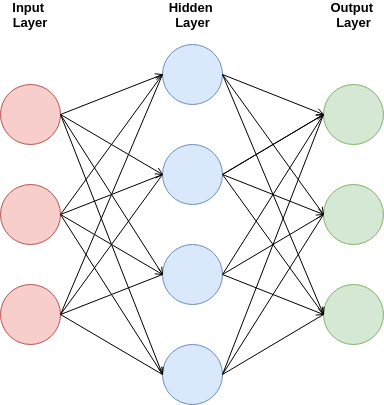
\includegraphics[scale=0.7]{background/figures/neural_network.png}
\caption{Simple illustration of a multilayer perceptron with three inputs, one hidden layer with four nodes, and one output layer with three nodes.}
\label{fig:mlnn}
\end{figure}

Figure \ref{fig:mlnn} shows the basic structure of a multilayer network.
In this figure, we have four things we need to look into.

\subsection{Feed forward and backpropagation through a neural network}
\todo{looked at how MLP works, let us look at back-and-forward prop}





    
\subsection{Convolutional neural networks}
The multilayer perceptron we have discussed is a strong tool that can learn a multitude of decision boundaries, and subsequently learn to classify thousands of different classes. 
As we get more data and more classes, the networks needed to solve our problem grows. We can recall from chapter \todo{ref chapter on MLP} that the number of weights between neurons is \todo{insert math}. As the number of perceptrons per layer in our neural networks increases, the total amount of storage space increases by a factor of 4 \todo{fix this}

Another problem with the standard MLP is the fact that it is spatially dependent. Given an input $x$, the output, $y$, of the MLP will vary a lot if we shift the input data by one place, or if we flip the data. In some cases, this is something we want in our machine learning algorithms, but more often than not, this behaviour is not a desirable outcome.

Given the downsides we have with regards to memory usage and non-spatiality in our multilayer perceptrons, we present Kunihiko Fukushima \todo{cite} solution to solve both complications.

Convolutional neural networks are the most popular form for image recognition, segmentation, and classification \todo{cite, IEEE paper got cites}

When building a convolutional neural network we often use multiple layers stacked on opt of each other to give the network traits that a regular multilayer perceptron could not achieve. By far the most essential layer of the convolutional neural network is the convolutional layer.


\subsubsection{Convolutional layers}

Convolutional networks work with filters as opposed to perceptrons with weights assigned before and after the input in the vertices between perceptron. Convolutional layers assign a weight to each position in a special filter matrix. This use of filters significantly reduces the number of weights between layers, since we now have weights that are not dependent on the input size, and only dependent on this matrix size.

The three main parameters of a convolutional layer are the number of filters, kernel size and strides.
When making a convolutional layer, we start by pseudo-randomly initialising a $ (F \times K \times K)$ matrix as our weights.
In this matrix, F is the number of filters in the convolutional layer and K is the filter size. We can think of this as F filters of size $(K \times K)$ stacked on top of each other. 
When applying the convolutional layer to an input vector, we take each of the F filters and slide it over the image. 
For each position of the filter, we multiply the image value with the filter and sum the result. The scalar made by this multiplication is the value passed on to the next layer at that specific point.
Figure \ref{fig:conv_opp} shows the this convolution process after 3 sliding operations with a $(3 \times 3)$ filter.
 
\begin{figure}[t]
        \centering
        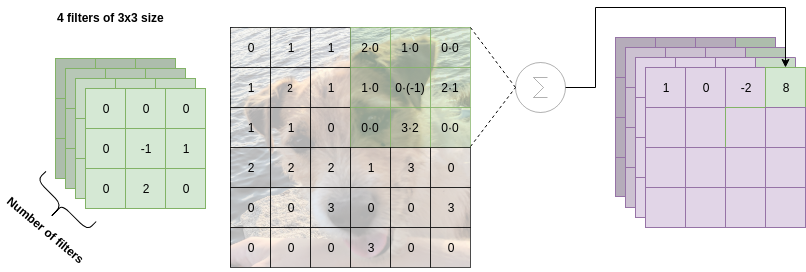
\includegraphics[scale=0.5]{background/figures/Conv_filter.png}
        \caption{The values calculated when a convolutional filter after 4 sliding window operations, here the number of inputs does not represent how many inputs there usually is in an image}
        \label{fig:conv_opp}
\end{figure}


As we can see from this architecture, we can only change when weights in the filter matrix, as there are no other variables in the convolutional operation. Using this sliding window technique gives us the benefit that the filter only gathers information from the local area, and subsequently makes the convolutional operation non-spatially dependent.  

\subsubsection{Activation layers}
As we discussed in chapter \ref{chap:perceptron}, in addition to summing the inputs and passing them on, we need to apply an activation function to the output. The same problem with our desire to make non-linear problems apply in the CNN model. 
To apply an activation layer to a CNN, we take every value in the matrix and apply the activation function separately to every data-point. 

\subsubsection{Pooling}
Pooling layers, often also called downsampling layers, are commonly also found in CNN's. 
Their primary role in the network is to reduce the spatial size of the data provided, and thus reducing the number of weights and variables used by the network.  
The two most common pooling operations are max pooling and average pooling\todo{cite}. Both methods resemble convolutions in the way that they apply their function to a sliding filter over the data. 
 
\begin{figure}[h]
        \centering
        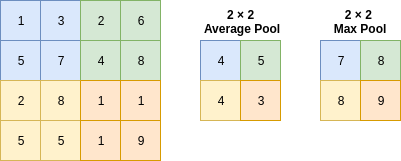
\includegraphics[scale=0.7]{background/figures/pooling.png}
        \caption{Both max and average pooling done on a 4 $\times$ 4 matrix}
        \label{fig:pooling}
\end{figure}

Just like in Figure \ref{fig:pooling} the most common pooling parameters are of filter size 2 and stride 2. Using this configuration leaves every point of the input checked once, and the resulting output size is halved. 
Pooling layers do generally not have any weights associated with them. This lack of weights means that the pooling layer routes the signal back without changing it during backpropagation.
\todo{unpooling}

\subsubsection{Normalisation}
Normalisation layers are one of the newer addition to the CNN models. The normalisation layers, as with the pooling layers does not contain any weights, ad subsequently only change the data based on the statistics of the data. 



In CNN models the most used type of normalisation is batch normalisation.

\begin{itemize}
\item Learning faster
\item Increase Accuracy
\end{itemize}




\subsubsection{Dropout}
A major problem in machine learning is the act of overfitting the data. We say that a model is overfitting to the data when it learns the bias that comes with the dataset. 
 
\begin{figure}[h]
        \centering
        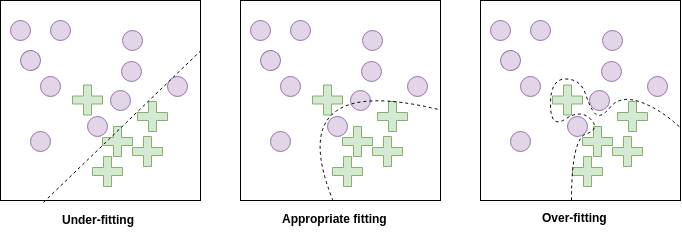
\includegraphics[scale=0.6]{background/figures/Under_vs_overfitting.png}
        \caption{Three cases of data boundary prediction. In most cases we desire appropriate amount of fitting to our dataset to keep generalisation}
        \label{fig:dropout}
\end{figure}


Dropout, first proposed by Srivastava et al.\cite{JMLR:v15:srivastava14a}, in 2014 was used to prevent overfitting of neural networks (As seen in figure \ref{fig:dropout}).
Dropout layers in the CNN will randomly cut a certain amount of connections in a layer. The amount is usually between 25\% and 50\% of the connections. The result of the use of dropout is that the network can not rely on only a few numbers of weights during training since there is a chance the input from the weight will be cut at random intervals. 

This random cutting forces the network to spread out the essential weights throughout the network. 
Even though dropout does not explicitly change the weights, it implicitly forces the stong weights to be eavenly distributed throughout the network. 
Dropout does, in practice, the same as an L1 or L2 regularizer. 



\section{Complex Neural Network models}
We have looked at the basic concept of the neural network, and a more in-depth look into the convolutional neural network and the relevant layers.
Our primary focus has been from a computer vision perspective, where we have looked at image classification. 
To get a better insight into the act of inpainting, we need to present two other types of network, namely the Autoencoder \cite{Rumelhart:1986:LIR:104279.104293} and the generative adversarial network \cite{Goodfellow:2014:GAN:2969033.2969125}.

We often base both models on the convolutional architecture, to have the option to work with image and video data. 
Both networks are a type of unsupervised learning, where the goal is to either recreate or construct data based on the training data.



\subsection{Autoencoders}
\label{cha:Explaining_autoencoders}
 An autoencoder is a neural network that is trained to recreate a copy of the input given. 
As with the networks explained at this point, it has an input, some number of hidden layers and an output. The network can be considered to have two internal structures, the encoder (denoted as $h=f(x)$) and decoder (denoted as $r=g(h)$) shown in figure \ref{fig:simpleAE}.
The general goal of the autoencoder is to recreate the input $g(f(x)) = x$, but in the real world, we often add restrictions to make the autoencoder unable to copy the input perfectly. Because of this restriction, the autoencoder is forced to prioritise particular properties of the data. Figure \ref{fig:simpleAE} shows the general structure of the autoencoder.

\begin{figure}
    \centering
    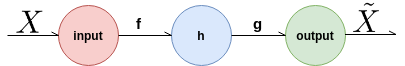
\includegraphics[scale=0.6]{background/figures/SimpleAE.png}
    \caption{The general structure of an autoencoder, encoding $\textbf{x}$ with $\textbf{f}$, then decoding $\textbf{h}$ with $\textbf{g}$ to an output $\textbf{x}$.}
    \label{fig:simpleAE}
\end{figure}

Traditionally, autoencoders were used for tasks like feature learning and dimensionality reduction, though with the rise in computing power, autoencoders are now in use at the forefront of generative modelling.


To use an autoencoder for generative modelling, we need to set an objective for autoencoder to achieve.
A when generating new images we can propose regulisers to the latent space between the encoder and the decoder. The reguliser might be that the output of the latent space layer should follow a Gaussian noise pattern. 
This type of autoencoder is called a variational autoencoder. Variational autoencoders have the advantage of being able to create new completely unseen data if Gaussian noise is inputted at the latent space, effectively cutting out the encoder and supplying random noise instead.



Another way to use an autoencoder for generative modelling is by masking areas in the input data the model used to train on, and give the unmasked data as the target output.
Figure \ref{fig:AEinpainting} shows the general concept of an inpainting Autoencoder.



\begin{figure}
    \centering
    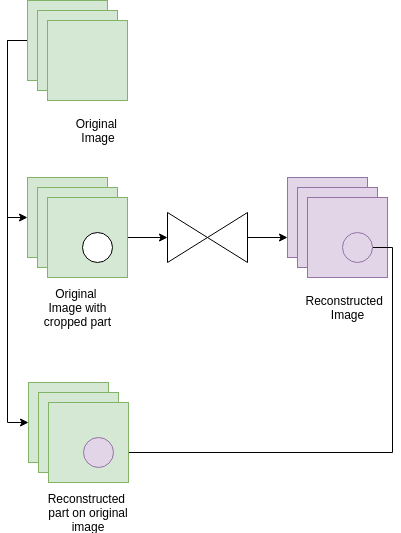
\includegraphics[scale=0.6]{background/figures/AE_for_inpainting.png}
    \caption{Autoencoder where the goal is to inpaint the masked area}
    \label{fig:AEinpainting}
\end{figure}



As with supervised classifiers, autoencoders use gradient descent to optimise  the result, as the model work to recreate the input $\textbf{x}$ from out output $\widetilde{\textbf{x}}$\\    
We achieve this by minimising the loss function:\\
\begin{equation}
    \mathcal{L}(\textbf{x},g(f(\textbf{x})))
    \label{eq:AEloss}
\end{equation}
As this is a problem where the goal is to minimise error, autoencoders often use mean square error or mean absolute error as the optimiser for the gradient descent. 
Figure \ref{fig:AEinpainting} show a visual example of equation \ref{eq:AEloss}.


    
\subsection{Advaserial neural networks}
\paragraph{This is explaining GANS, put me in the right place} %%TODO CITE: http://www.deeplearningbook.org/contents/generative_models.html and Goodfellow at al. 2014

Now that we have looked at autoencoders we can take it a step further. 
generative adversarial models can be used as a generator of new data and can have some resemblance to autoencoders \ref{Explaining_autoencoders}, especially variational autoencoders. \cite{Goodfellowetal2016} %TODO cite VAE, ref VAE

The difference lies in that adversarial networks is based on game theoretic scenarios in which a generator network is competing against an advasery. 
The generator produces samples $x=g(z;\theta^{(g)})$, where $g$ is the network given the weights $\theta$. Then the discriminator network predicts if a sample is drawn from the dataset or from the generator.
More spessific, it gives a probably given by $d(x;\theta^{(d)})$ , and determines if $x$ is from the generator or the data-set. 
Since we have two networks competing against each other we can look at this as a Zero-sum game with the generators payoff is determined by $v(\theta^{(g)},\theta^{(d)})$, and the discriminators payoff is determined by $-v(\theta^{(g)},\theta^{(d)})$.
\textit{$v$ is here a function that is determined by both the success rate of the discriminator and the generator, the most commonly used is}
\begin{equation} %TODO: CITE First gan paper on formula
    v(\theta^{(g)},\theta^{(d)}) \; = \; \mathds{E}_{x\sim p_{data}}\log{d(x)} + \mathds{E}_{x\sim p_{model}}\log{(1 - d(x))} 
\end{equation}
as derived from Goodfellow et al. %TODO cite 
      
Lets look at a gan in detail. \\
\begin{figure}[ht!]
    \centering
    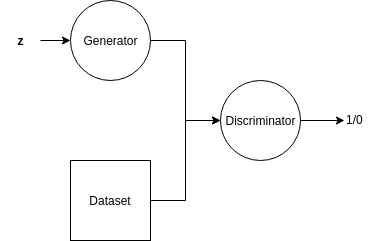
\includegraphics[scale=0.5]{background/figures/simpleGAN.png}
    \caption{The idea behind a GAN. Here the generator samples from a random (Gaussian) distribution and generates samples that the discriminator classifies as real or fake}
\end{figure}
    
%\subsection{Recurrent neural networks}
%\subsection{LSTM}

\subsubsection{Contextencoders}
Inpainting can also be done with adversarial models, and using a network trained to do the task of inpainting can be a lot more powerful than using just an autoencoder\todo{ref} or the naive methods\todo{ref}.
A contextencoder is building on the adversarial principle by using a generator/discriminator pair to fill in masked areas in an image. 
    
The concept behind a Contextencoder is to take the whole image as input to an encoder/decoder pair and \todo{finish}
     
\subsubsection{CC-GANS}  
%\subsection{Pixel CNN}
      
    



        
   
\section{The problem at hand / Summary}
      
\subsubsection{Explain how the ML-methods can be used with the polyps}
    When you work with machine learning a lot of the job is to make the data as clear as possible. \\
    Imagine that you want to do something as simple as reading an analogue clock. The \"straight forward\" way to do it is to make a convolutional neural network to look at the dials. This will require a much more complex network compared to if you could convert the angle of the dials to degrees and have that as an input to your model.

    \begin{figure}[ht]
      \centering
      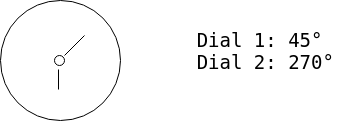
\includegraphics[scale=0.5]{methods/figures/Clock.png}
      \caption{A clock needs a more complex network compared to just the degrees}
    \end{figure}
    %TODO FIND ORIGinal source
    The trick is often to make the data as refined as possible. 
    Further, some of the techniques used are described.
    
    \todo{Here I need to talk about how preprocessing might help the problem, and make this a springboard into the next section: the problem at hand}
    
    
    \todo{adress the problem with lack of data, and talk about how machine learning can help, machine learning.}
      
   




\begin{itemize}
	\item Stevens paper about inpainting
	\item Konstantins paper about the cross dataset evaluation
\end{itemize}



      Now that we have the definition of machine learning and the current task, we can focus on the task at hand; finding polyps. In an ideal world\footnote{Ideal as in the only disease, we could get in  the GI tract was cancer originating
      from polyps which looked exactly the same} we have a
      Classification problem with only two classes: Non-polyp and polyp. 
      
      \begin{itemize}
        \item SVM 
        \item CNN 
        \item random forests
        \item knn
      \end{itemize}


















































\iffalse
\section{In painting}
  We have discussed the importance of good input data, and the potential benefits to resource usage and ease of making a good model.
  So a priority when it comes to image classification is to have data without anomalies and other areas that can be interpreted as a feature for the classifier. 
  In a machine learning perspective, the data is best if it has the same structure, and is %TODO similar enough.
  In painting is the process of reconstructing lost or deteriorated parts of images and videos. %TODO CITE https://en.wikipedia.org/wiki/Inpainting
  

  From previous papers on polyp detection in the GI tract %TODO CITE!!!
We have clear results that the black corners and the green squares trigger a big activation %TODO WRITE BETTER
  when it comes to classifying images. 
  From %TODO CITE, find out who
  's paper, we can see that the activation map on a regular image gives a very high result on, in addition to the polyp, the corners and the green square. 
  \begin{figure}[ht]
    \centering
    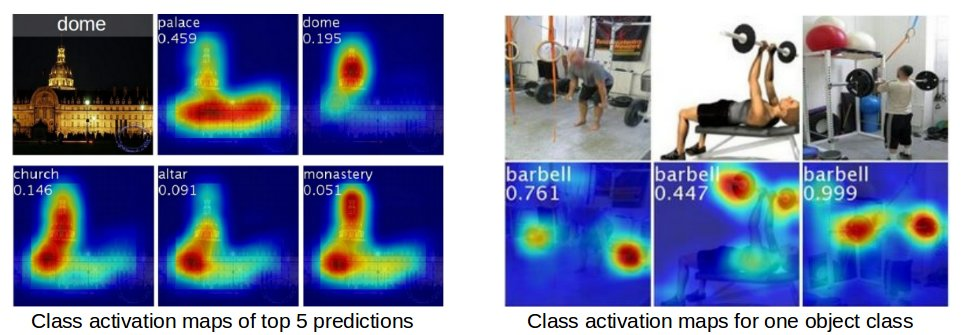
\includegraphics[scale=0.5]{background/figures/placeholder.jpeg}
    \caption{Using X's activation map we can see that the edges triggers unwanted activations}
  \end{figure}
  
  In addition to squares and edges, we also have the problem that parts of the image is over saturated at points where the light from the led is reflected directly back to the camera.
  Another problem is when the camera captures images that are too close to the wall. Both of these scenarios creates patches where the saturation is maximum. 
   \begin{figure}[ht]
    \centering
    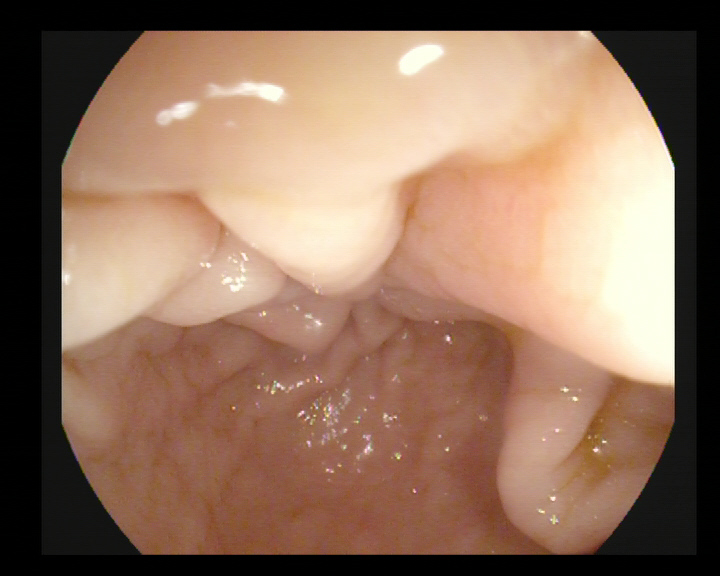
\includegraphics[scale=0.5]{background/figures/reflection.jpg}
    \caption{we have two different types of saturation: the reflected area in the top part of the image, and the right side of the image.}
  \end{figure}
  in an ideal scenario, the image would have no pixel values at max, and as little frame as possible. 
  We, therefore, want to make a tool that can help us with this.
  \subsection{Naive methods for In painting}
    Inpainting is not a new area of research, as it has been around since %TODO CITE
    Because of this, there are many naive methods that give good inpaintings. 
    
    \subsubsection{Textured syntesys based on image inpainting}
    \subsubsection{MOARE}
    \subsubsection{MOARE}
   \subsection{Naive methods for borderfinding}

%
% THIS SECTION MUST BE MOVED/FIXED
%
\section{Naive Methods REM}
      Now that we have an idea of what we are looking for we can first turn to some more naive methods for detecting anomalies, and for enhancing the images.\\
      The field of image processing has been researched since\\ %TODO WHEN
      
      Using some of the classic methods in image processing, we can see if\\ %TODO
      
      We often describe the method into two groups of information: First and Second order statistics.\\
      \textbf{First order:} First order statistics does not take in to account the relative positioning of the pixels in the image, and because of this, gives much less information than the second order statistics.\\
      Example of First-order statistics is often what information we can get out of a histogram. This can be skewness, variance, and mean value.\\
      
      \vspace{10px}
      
      \textbf{Second order:} Second-order statistics takes in to account the relative positioning of the pixels in the image. We can calculate the GLCM matrix and get a much more detailed view of the image. \\
      
      
      
      \subsection{GLCM}
        A GLCM (Grey-level co-occurrence matrix) is a matrix that is used when examining the spatial relationship of pixels in a texture. 
        The calculation of a GLCM gives us how often pairs of pixels with specific values and a specified spatial relationship occur at a given place in an image. %TODO CITE
      
        \subsubsection{Algorithm}
          For simplicity we use only greyscale in this example:
          \begin{figure}[ht]
        \centering
        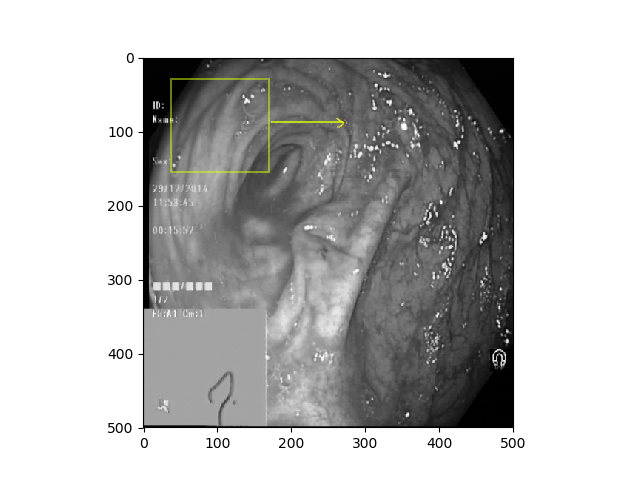
\includegraphics[scale=0.5]{figures/sliding_window_box.png}
        \caption{GLCM capturing features}
          \end{figure}
          The algorithm starts by running a sliding window over the image, often with a stride, and for each stop calculates the spatial relationship between each pixel specified.
          The result can be something like this figure %TODO link to figure
          where we can read out the most likely neighbouring pixel.
           \begin{figure}[ht]
        \centering
        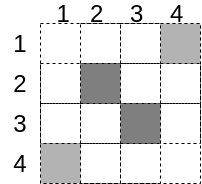
\includegraphics[scale=0.5]{figures/Simple_GLCM.png}
        \caption{GLCM Matrix}
          \end{figure}
          The darker colours on in the matrix are indicating that we often have a jump between, for instance, pixel-value of 1 and a pixel value of 4, but no from 1 to 1.\\
          With this information, we can get a naive pattern-recogniser. 
        \subsubsection{Other uses}
          Besides for the pattern recognition we can use the GLCM to get the information on:
          \begin{itemize}
           \item \textbf{Contrast} is the difference in luminance or colour in the picture. We would expect low contrast in the “background” and higher contrast around edges and irregular objects.
           \item \textbf{Homogeneity} is how similar a local area is to itself
           \item \textbf{Variance} $\sigma^2$ , is directly a measure of ”roughness”
           \item \textbf{Mean} value of a GLCM can give us areas with higer or lower pixel values. Good way to find polyps if they are lighter than the tissue around.
           \item \textbf{Entropy}
           \item \textbf{Energy}
          \end{itemize}


      
      \subsection{Edge detection}
        Using Edge detection in is another viable way to look for polyps. 
        \begin{figure}[ht]
          \centering
          \begin{minipage}[b]{0.45\textwidth}
        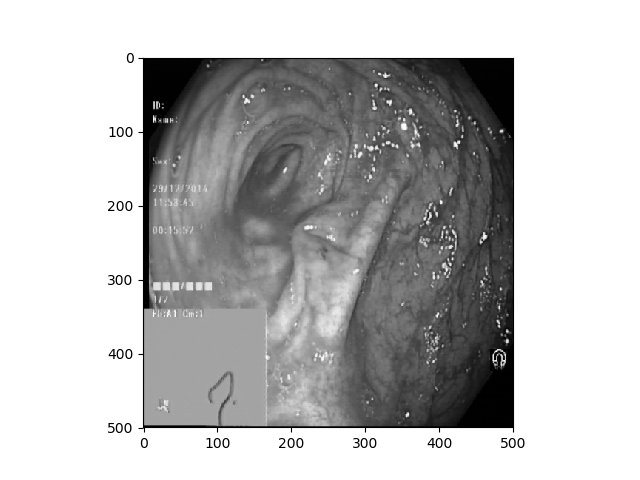
\includegraphics[width=\textwidth]{figures/sliding_window.png}
        \caption{Original image}
          \end{minipage}
          \hfill
          \begin{minipage}[b]{0.45\textwidth}
        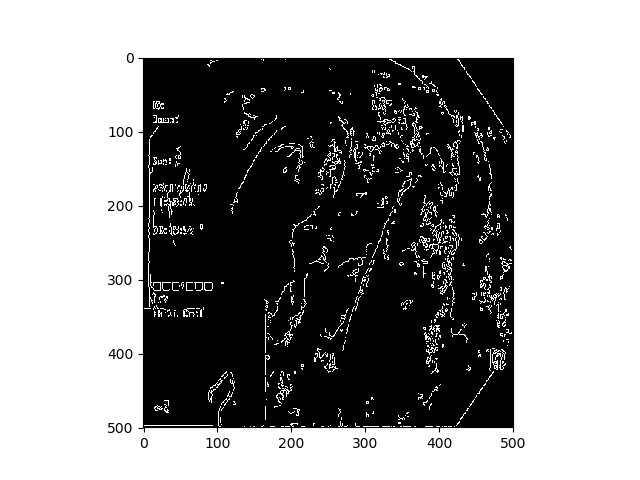
\includegraphics[width=\textwidth]{figures/Canny.png}
        \caption{Edges of the picture}
          \end{minipage}
        \end{figure}
        \subsubsection{Algorithm}
          For each pixel look at the neighbouring pixel, if \\
          
          \begin{centering} 
        $ abs(p_a - p_b)>tresh $\\ 
          \end{centering}
          
          then mark a pixel as an edge pixel. \\
          
      \subsection{Hough Transforms}
        Using, for instance, Canny edge detection %TODO CITE
        we can get a better view of where the potential border of the polyp/anomaly is. (As shown in %TODO FIG CITE)
        
        A Hough transform can I theory have many/any shape(s), and together with edge detection, we might find some of the polyps this way.
        
    
    
    
    
    
    
    As we can see from this, there are a lot of old methods that can give approximations. We can also conclude that none of these methods is perfect.
    We will, therefore, look at methods that take learning in to use.
\section{Using machine learning for inpainting}
    \subsection{AE}
    \subsection{CE}
    \subsection{CCGAN}
    \subsection{PCNN}
    As discussed earlier, machine learning is using prior experiences to make decisions given the problem at hand. 
    It is also worth mentioning that we do not need labelled data since we are in a way looking at a global average of every image both with and without polyps. We are therefore incentivised to use an 
    Unsupervised approach.
    Since machine learning is learning from a training set, it is essential that the training set contains as little as possible of the features we want to remove. \\
    
    Because of this, the first thing we need to do if we are going to mask out corners and squares is to limit the training set only to contain cropped, non-square images. 
 
    \begin{figure}[ht]
      \centering
      \begin{minipage}[b]{0.45\textwidth}
    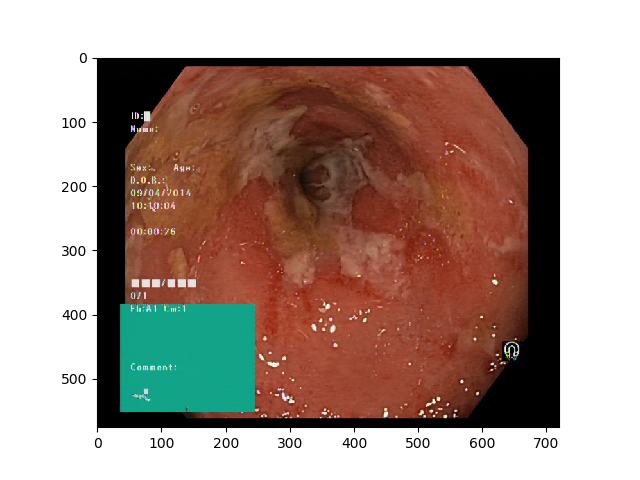
\includegraphics[width=\textwidth]{background/figures/uncropped_img.png}
    \caption{Original image with black padding}
      \end{minipage}
      \hfill
      \begin{minipage}[b]{0.45\textwidth}
    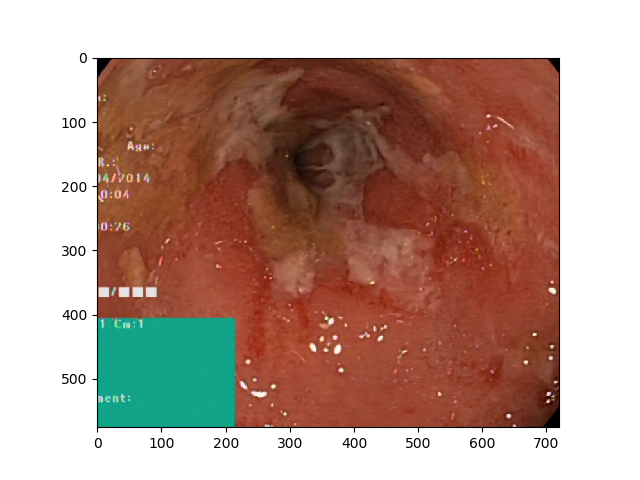
\includegraphics[width=\textwidth]{background/figures/cropped_8percent_img.png}
    \caption{Black edges cropped away + 8\% zoom}
      \end{minipage}
      \caption{Here we have an example on how we would make an image better to train on. This is not representative of the training since we only use images without the green square under training}
    \end{figure}
    
    Now that we have better images to train our data with, we need the correct algorithm.
    We have already seen unsupervised learning aproaches in chapter %TODO ref 
    \newpage
    \subsubsection{Algorithm}
      \todo{Hvordan skal jeg gaa frem nar det kommer til aa presantere disse? skal jeg bare si hvilke metoder jeg har testet?}
      Text about presenting UML, and stuff.
  
    \newpage
    As we recall from earlier, an autoencoder is a type of neural network that tries to output a recreation of the output.\\%TODO: REF the part about autoencoders 
    We can use this for inpainting by setting the algorithm to train on images with areas cropped away.
    There are a couple of different ways we can train an autoencoder to do this.\\
    
    %\todo{shouldI talk about the different ways or present the best?}
    
    
    \vspace{10px}
    \textbf{Denoising Autoencoder with MSE loss:}\label{par:Denoising_Autoencoder_with_MSE_loss}\\
    The simplest way to train the autoencoder is to first take the trainingset $\mathds{X}$ and make an augmented copy $\widetilde{\textbf{x}}^{(i)}$ for 
    every data point in $\textbf{x}_{\sim \mathds{X}}^{(i)}$. \\
    \textit{Here $\widetilde{\textbf{x}}$ is a copy of x with random areas masked.}\\
    
    Now we minimise the loss function\\    
      \begin{equation}
        L(\textbf{x},g(f(\widetilde{\textbf{x}})))
      \end{equation}
    over the whole image.\\
    \vspace{20px}
    
    With this approach, the autoencoder learns to fill in the blank spots with credible data, without changing the rest of the image. 
    \todo{this will probably work best if the autoencoder is not under complete, perhaps talk about this}
    One problem by this approach is that we do not want the rest of the image to change for obvious reasons, and the algorithm as it is here has the flaw that it will change all the pixels in the image, at least to a minor degree. \\
    
    This can be somewhat fixed by only taking the augmented parts, and pasting them directly into the image. This will leave most of the original image, except for the parts that were cropped randomly.\\
    
    \vspace{10px}
    \textbf{Denoising Autoencoder with \todo{clever tittle}:}\\
    If we take what we learned from \ref{par:Denoising_Autoencoder_with_MSE_loss}, we can make a more optimal autoencoder:
    Rather than taking a loss like     
    \begin{equation}
      L(\textbf{x},g(f(\widetilde{\textbf{x}})))
    \end{equation}
    over the whole image, we can rather just focus on the parts that matters, namely the cropped areas.\\
    
    If we add the cropped image to the output from the autoencoder to make an image, we can use this new image to train out loss.
    For most of the image, the loss will be zero, since the only part that is changed is the cropped area. 
    We can also make a new loss that is more optimal for the task at hand. 
    \begin{equation}
      MSE_{crop}\:=\: \frac{1}{n}
      \begin{cases}
          \begin{array}{lcl}
          (\widetilde{\textbf{x}}-\textbf{x}) \; if \; \widetilde{\textbf{x}} \: \in \: \textbf{x}_{crop} \\
          0 \; else
          \end{array}
      \end{cases}
    \end{equation}
    Where $\textbf{x}_{crop}$ is the area that was cropped away from the original image and $n$ is the number of pixels in that area.\\
    With this modified MSE we are assured that only the pixels in the cropped area is changed with gradient decent, and we save a lot of computation as an added bonus.
    
    
    \todo{token to not train}
    \begin{figure}[ht!]
        \centering
        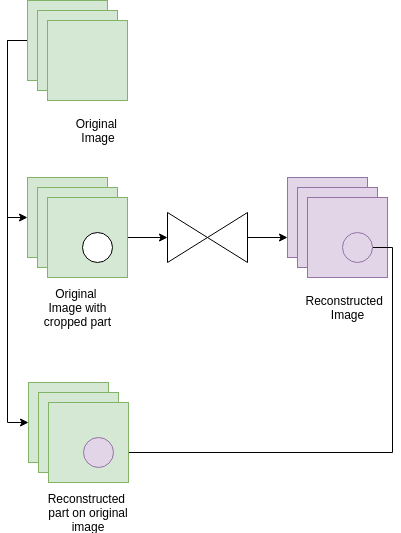
\includegraphics[scale=0.5]{background/figures/AE_for_inpainting.png}
        \caption{Final result of the autoencoder used in the testing}
    \end{figure}
    
    
    
    
    
      \subsubsection{Explaining GANs, this will be moved}
      
    
      \subsubsection{Contextencoder}
    Inpainting can also be done with adversarial models, and using a network trained to do the task of inpainting can be a lot more powerful than using just an autoencoder\todo{ref} or the naive methods\todo{ref}.
    A contextencoder is building on the adversarial principle by using a generator/discriminator pair to fill in masked areas in an image. 
    
    The concept behind a Contextencoder is to take the whole image as input to an encoder/decoder pair and \todo{finish}
    
    
    
      \subsubsection{CCgan}
      \subsubsection{PixelCNN}
      
\fi

  
 
